\chapter{Implementation des Indexers}

Ein Teil der Arbeit war es, einen Indexer zu implementieren, der die Dateien des Benutzers durchl�uft und - wie es der Name vermuten l�sst - interessante Dateien indexiert. In diesem Kapitel soll auf den Aufbau und die Implementationsdetails eingegangen werden.

\section{Aufbau}

Der Indexer ist als parallelisiertes, knotenbasiertes System konzipiert worden. Die Parallelit�t wurde deshalb gew�hlt, weil es beim Einholen der verschiedenen Datenquellen teils zu Wartezeiten kommt, die gut anders genutzt werden k�nnen. Dieser Faktor kam besonders ins Spiel als noch zus�tzlich zu den Musikdaten auch Bilderdaten gesammelt worden sind.

Ein weiterer Grund f�r die Parallelisierung ist, dass als m�gliches Feature eine real-time Indexierung vorgesehen war, die es letztendlich allerdings nicht in das fertige Programm schaffte.




\section{Datenquellen}

Da IMVR zum Ziel hat, die Musik des Benutzers in verschiedenen Formen und Farben darzustellen, werden Daten von diversen Quellen ben�tigt. Wir leben in einer wundervollen Zeit in Sachen Datenvielfalt: Es gib viele Online-Services, welche zu einem Grossteil gratis sind, von denen man diverse Daten erhalten kann.

Es folgt eine kurze Zusammenstellung von untersuchten Datenquellen.


\begin{table}[H]
\caption{Eine �bersicht von verf�gbaren Online-Datenquellen.}
\centering
\label{t:datasources}
\begin{tabular}{ l l l }
	\noalign{\smallskip} \hline \hline \noalign{\smallskip}
	\textbf{Name} & \textbf{Daten} & \textbf{API-Limite} \\ \midrule
	Last.fm & Bilder, Meta-Daten & 1 Request / Sekunde \\
	The Echo Nest & Bilder, Meta-Daten, Analyse-Daten & 120 Requests / Minute \\
	Spotify & Bilder, Meta-Daten, Playlisten, Streams & ? \\
	Amazon & Bilder, Beschreibungen & 1 Request / Sekunde \\
	Gracenote & Bilder, Fingerprinting, Meta-Daten & $\sim$1000 Requests / Tag \\
	MusicBrainz & Bilder, Meta-Daten & $\sim$1 Request / Sekunde \\
	\noalign{\smallskip} \hline \noalign{\smallskip}
\end{tabular}
\end{table}

Im Falle von IMVR kommen die Daten grunds�tzlich von drei verschiedenen Quellen:

\begin{itemize}	
  \item ID3 Tags der Musik-Dateien
  \item The Echo Nest
  \item Last.fm
\end{itemize}

Diese wurden gew�hlt aufgrund der durchsichtigen API-Limite und den verf�gbaren Daten. The Echo Nest aggregiert zudem die Daten von anderen Seiten wie Spotify und MusicBrainz, und enth�lt wertvolle Analyse-Daten, die in eine zentrale Position in IMVR haben.

\begin{figure}[h]
\centering
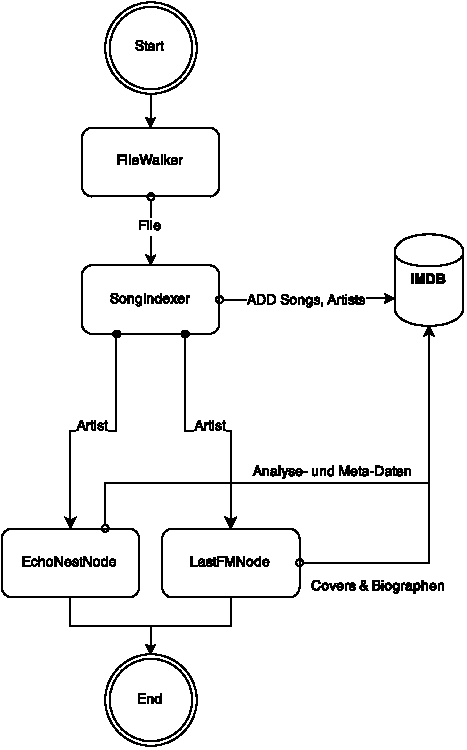
\includegraphics[width=0.5\linewidth]{bilder/Indexer-DataFlow.pdf}
\caption{Der Datenfluss, den die Files beim Indexieren nehmen.}
\label{fig:Indexer-DataFlow}
\end{figure}


In einem ersten Schritt werden grundlegende Daten wie der Titel des Liedes, der Name des Artisten, usw. aus der Datei selbst entnommen. Wenn m�glich wird auch gleich gepr�ft, ob ein Album-Cover hinterlegt ist.

In einem zweiten Schritt wird �ber eine .NET Bibliothek, welche im Rahmen des Projektes geforkt und erweitert wurde, zur API von The Echo Nest verbunden und diverse Meta-Daten zur Musik heruntergeladen.

\section{Datenstruktur}

F�r die Abspeicherung der Daten wurde zuerst ein Ansatz gew�hlt, der auf einer SQLite Datenbank basierte. Diese wurde in einem Prototyp auch erfolgreich implementiert. Es stellte sich jedoch heraus, dass diese Abh�ngigkeit das Programm unn�tig verkomplizieren w�rde und eine simple In-Memory Datenstruktur v�llig ausreicht.

Das finale Produkt verwendet also eine simple, objektorientiert Datenstruktur, die serialisiert und so zwischen den zwei Projekten (Indexer und IMVR) geteilt werden kann. Das Schema ist in Abbildung \ref{fig:Indexer-Commons} zu sehen. Damit beide Projekte Zugriff auf die genutzten Klassen haben, wurde das Schema in eine separate DLL ausgelagert, die ebenfalls als Abh�ngigkeit in beiden Projekten referenziert wird.

\begin{figure}[h]
	\centering
	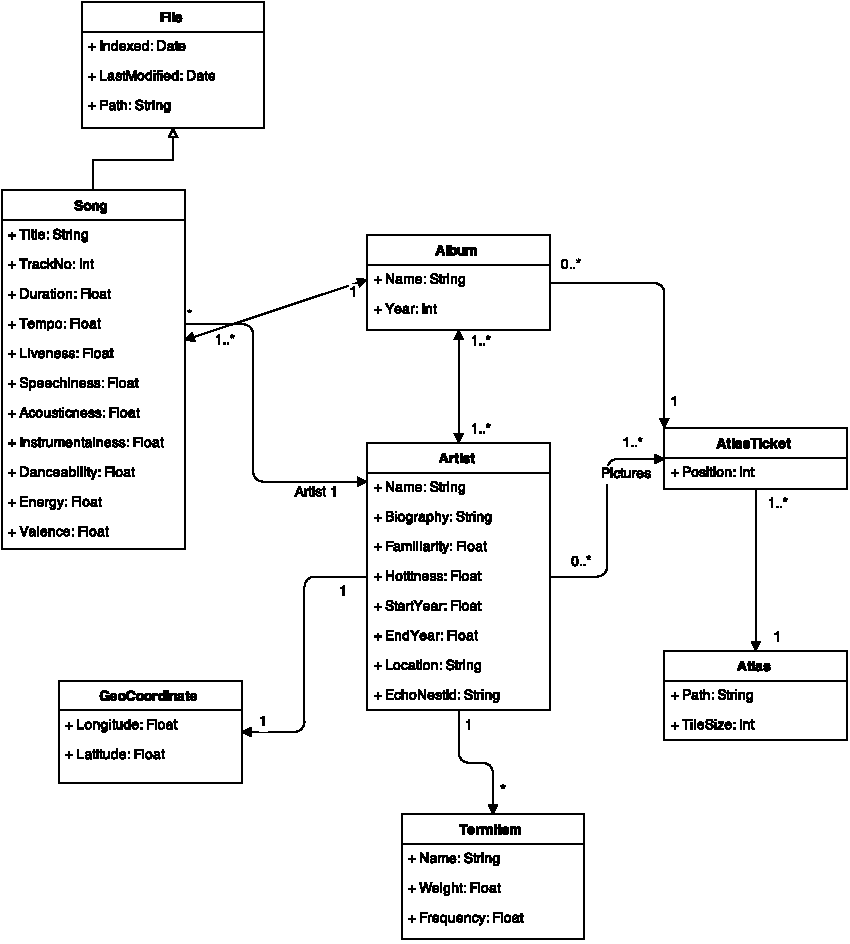
\includegraphics[width=0.7\linewidth]{bilder/Indexer-IMVR-Commons.pdf}
	\caption{Klassendiagramm f�r die Klassen im IMVR.Commons Package.}
	\label{fig:Indexer-Commons}
\end{figure}

Anzumerken ist, dass mehrere Einstiegspunkte auf die Daten existieren und so eine gewisse Redundanz geschaffen wird. Diese Redundanz ist hilfreich, weil in IMVR mehrere Modi eben diese Einstiegspunkte ben�tigen. Aufgrund der gew�hlten Serialisierungsmethode entsteht jedoch kein grosser Speicher-Overhead.

Die Serialisierung wird durch sogenannte Protocol Buffers \cite{wiki:protobufs} realisiert, wof�r eine Open-Source Bibliothek namens \textit{protobuf-net} \footnote{\url{https://code.google.com/p/protobuf-net/}} existiert. Protocol Buffers ist ein bin�res Datenformat, welches von Google Inc. entwickelt wurde und bekannt ist f�r seine Kompaktheit und Simplizit�t. Gew�hlt wurde es, weil die herk�mmliche Serialisierung mit .NETs \code{BinaryFormatter} zum Teil zu Problemen mit Unity f�hren kann.

\section{Herausforderungen}
